\documentclass[12pt, a4paper]{article}
\usepackage[utf8]{inputenc}
\usepackage[T1]{fontenc}
\usepackage[brazil]{babel}
\usepackage{geometry} % to change the page dimensions
\usepackage{graphicx}
\geometry{a4paper, left=3cm, right=3cm, bottom=3cm, top=3cm}

\begin{document}

\begin{figure}[htb]
\hspace{0.5cm}
\begin{minipage}[b]{0.3\linewidth}
    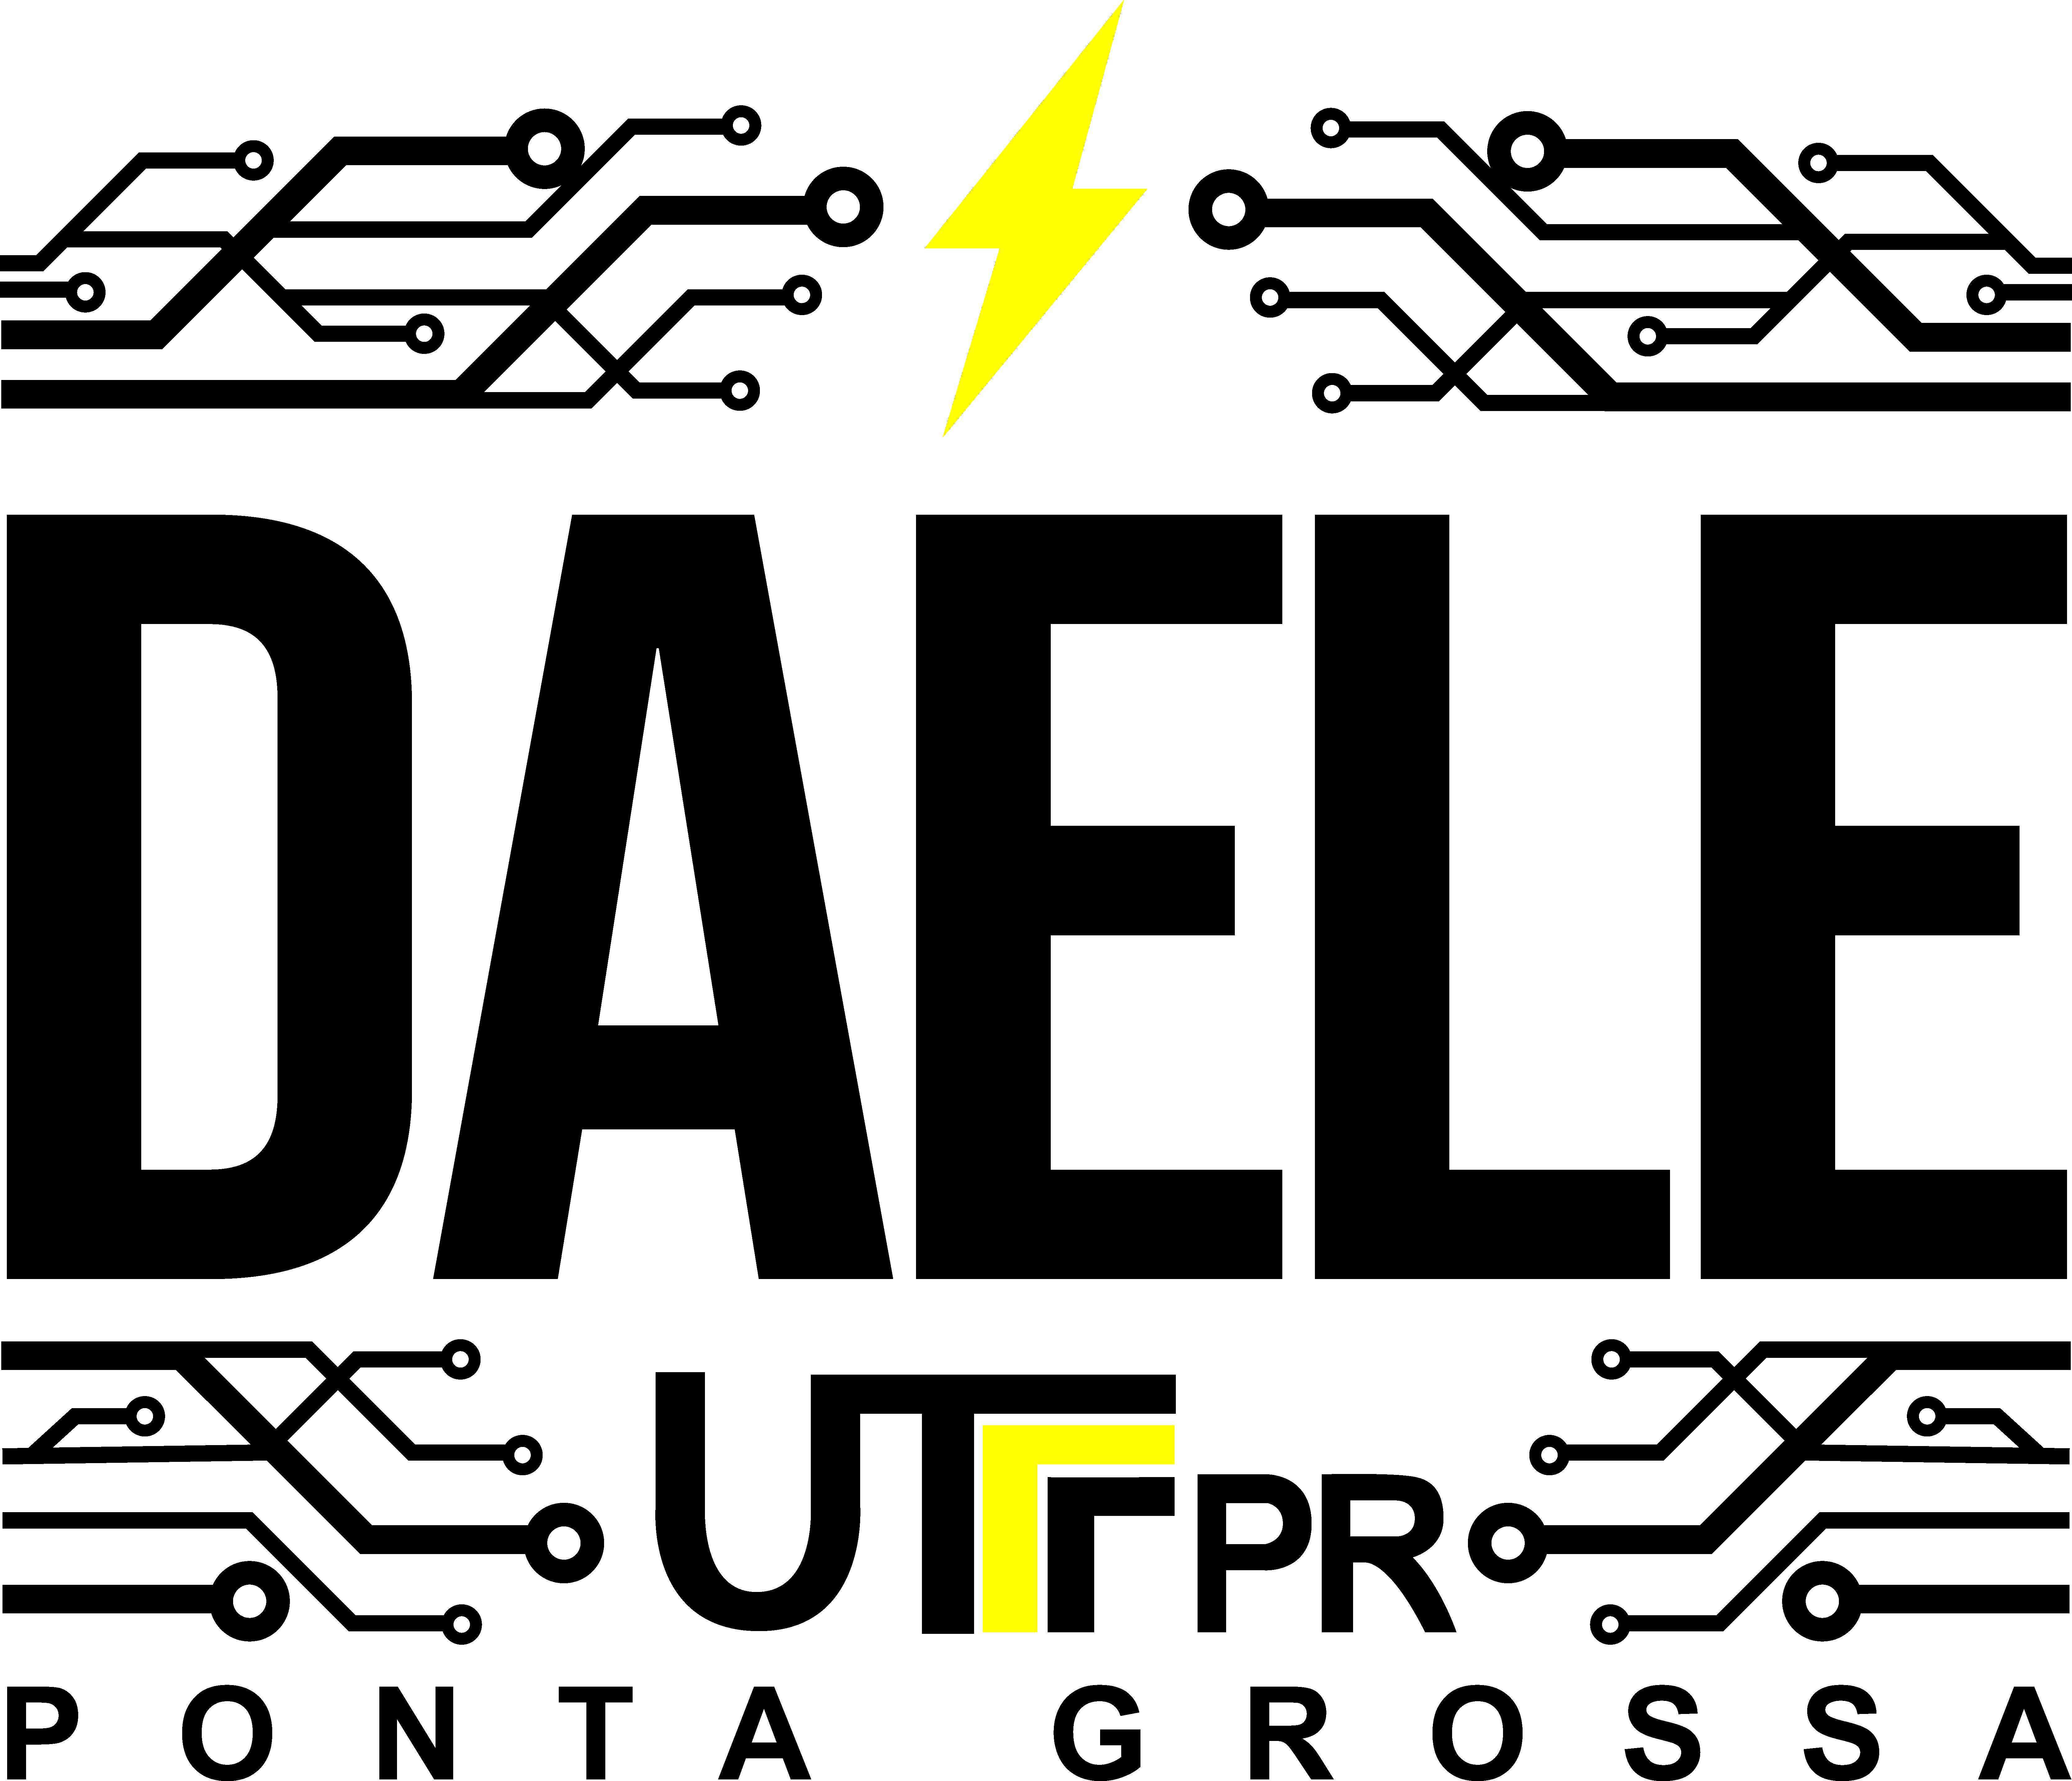
\includegraphics[width=4cm]{proj/logo.png}
\end{minipage}
\begin{minipage}[b]{0.65\linewidth}
\begin{huge}
Avaliação final TCC01.
\vspace{\baselineskip}
\end{huge}

\begin{Large}
Projeto do curso de TCC02.

\medskip 
\textit{Prof. \hspace{1.5mm}Dr. \hspace{1.5mm}Josmar \hspace{1mm}Ivanqui}
\end{Large}
\smallskip 
\end{minipage}
\end{figure}
\vspace{0.6\baselineskip}

Nome:\hrulefill
\vspace{\baselineskip}

Título do TCC:\hrulefill
\vspace{\baselineskip}

Orientador (se existir):\hrulefill
\vspace{3\baselineskip}


Sobre o TCC02, informar:
\vspace{0.8\baselineskip}

\begin{itemize}
    \item Qual o problema?\hrulefill
    \item Qual o objetivo geral?\hrulefill
    \item Quais são os seus objetivos específicos:
    \vspace{0.3\baselineskip}

    \hspace{0.6cm}– a)\hrulefill
 
    \hspace{0.6cm}– b)\hrulefill

    \hspace{0.6cm}– c)\hrulefill

    \hspace{0.6cm}– d)\hrulefill

    \item Qual a justificativa?\hrulefill
\end{itemize}

\vspace{-0.2\baselineskip}
\begin{table}[!h]
\caption{Cronograma previsto para o desenvolvimento do TCC 02.}
\begin{tabular}{|l|c|c|c|c|c|c|c|c|c|c|c|c|}
\hline
\textbf{Ano}     & \multicolumn{12}{c|}{\textbf{2020}}                                               \\ \hline
\textbf{Mês}     & jan. & fev. & mar. & abr. & mai. & jun. & jul. & ago. & set. & out. & nov. & dez. \\ \hline
\textbf{Fase 01} & x    & x    & x    & x    & x    &      &      &      &      &      &      &      \\ \hline
\textbf{Fase 02} &      &      &      &      & x    & x    & x    & x    & x    &      &      &      \\ \hline
\textbf{Fase 03} &      &      &      &      &      &      & x    & x    & x    & x    &      &      \\ \hline
\textbf{Fase 04} &      &      &      &      &      &      &      &      &      & x    & x    &      \\ \hline
\textbf{Fase 05} &      &      &      &      &      &      &      &      &      &      &      & x    \\ \hline
\end{tabular}
\end{table}

% Nao sabia se era pra deixar ou tirar

\noindent Tamanho: 12 pt. geral, também 25 pt e 20 pt
          
\noindent Margens: 3 cm (direita, esquerda, superior e inferior)
          
\noindent Espaçamento vertical: 1 cm.
          
\noindent Encaminhar o arquivo \textbf{tex} até o dia \textbf{06/12/2019}.


\end{document}
